\documentclass[../FinalThesis.tex]{subfiles}
\begin{document}
\setcounter{chapter}{-1}
\chapter{Additional Works}
\renewcommand{\thechapter}{A}
\thispagestyle{empty}
\vspace{-1cm}
\noindent\hfil\rule{0.75\textwidth}{.4pt}\hfil

\newpage
\section{Cameratrap Survey}
\label{CameratrapSurvey}

Our current understanding of AWD dispersal movements is primarily based on
models that consider landscape-scale information and environmental features
(e.g., water cover, vegetation cover, human influence) but are completely
uninformed with respect to the effect that intra- and inter-specific factors may
have. Recent studies have indicated that these factors may play a crucial role
in shaping dispersal movements, potentially even outweighing the role of
environmental factors, particularly in social species \citep{Cozzi.2018,
Armansin.2020}. To fill this data gap, I initiated a large-scale cameratrap
survey across BPC's historic study area (\Cref{Cameras}a). The goal of this
ongoing project is to obtain data on the distribution and abundance of AWDs'
main prey and competitor species, while also providing a non-invasive, long-term
monitoring system for the local fauna. Starting in November 2021, I deployed 60
cameras at as many stations on a 4x4 km raster grid, stratified by the three
predominant habitat types; grassland/floodplain (\Cref{Cameras}c), mixed
woodland acacia dominated (\Cref{Cameras}e), and mopane woodland
(\Cref{Cameras}d). To maximize the probability of detecting animals while
reducing our influence on the landscape, I placed cameras on trees
(\Cref{Cameras}b) facing dirt roads and programmed them to record bursts of four
images whenever an animal passed by.

\begin{figure}[htpb]
\begin{center}
  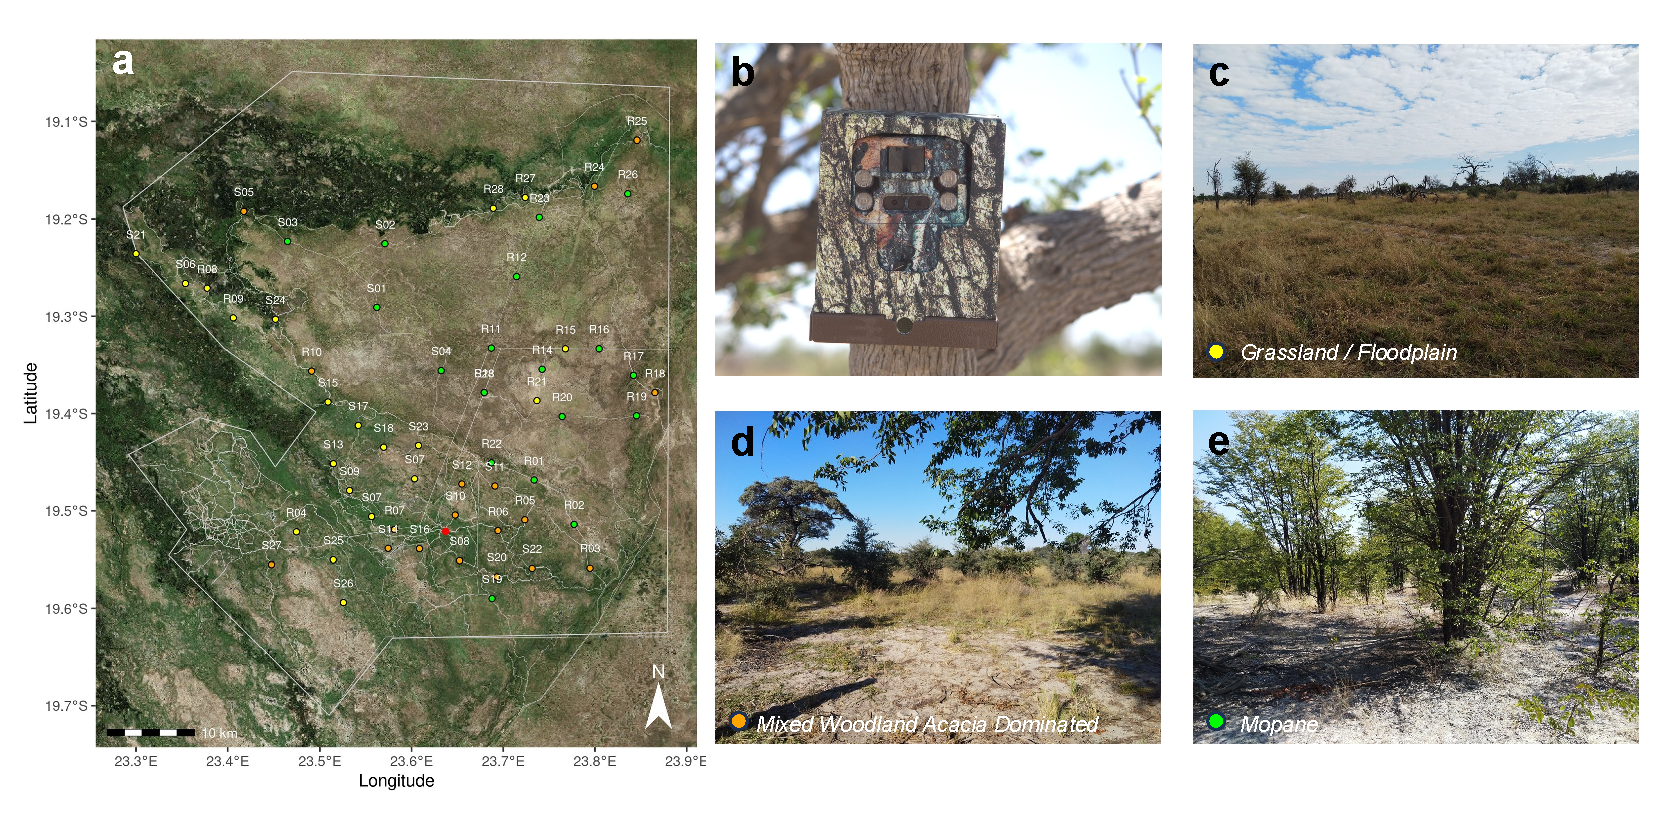
\includegraphics[width = 0.9\textwidth]{Figures/Cameras}
  \caption{(a) Camertraps deployed in BPC's historic study area. (b) Cameras
  were deployed on trees facing dirt roads and stratified across three major
  habitat types: (c) grassland / floodplain, (d) mixed woodland acacia
  dominated, and (e) mopane.}
  \label{Cameras}
\end{center}
\end{figure}

To cope with the large amount of incoming data, I developed a processing
pipeline that streamlines and automates numerous processing steps, thereby
reducing the need for manual labor (\Cref{CameratrapPipeline}). Notably, I
programmed a series of \texttt{R}-functions that allow pre-processing the
collected data using an object-oriented approach. Besides trivial tasks, such as
equalizing image dimensions or extracting EXIF-metadata, the functions also
allow feeding images into Microsoft's MegaDetector
(\url{https://github.com/microsoft/CameraTraps}). The MegaDetector utilizes an
AI model to separate images containing animals from those that are empty or
contain people and vehicles. This is particularly useful considering that
cameratraps are often triggered by moving vegetation, leading to false
positives. Finally, the data are automatically prepared for upload to Wildeye's
TrapTagger (\url{www.wildeyeconservation.org}) software for species
classification. In collaboration with Rapha{\"e}l Destriau (see
\Cref{Supervised}), this allowed me to classify animals on all 3.5 Mio.
collected images. As a follow-up from my doctoral thesis, I plan to use the so
collected and processed data to model the distribution of relevant species, and
to include the resulting layers as additional covariates in the dispersal models
that I developed and used thus far.

\begin{figure}[htpb]
\begin{center}
  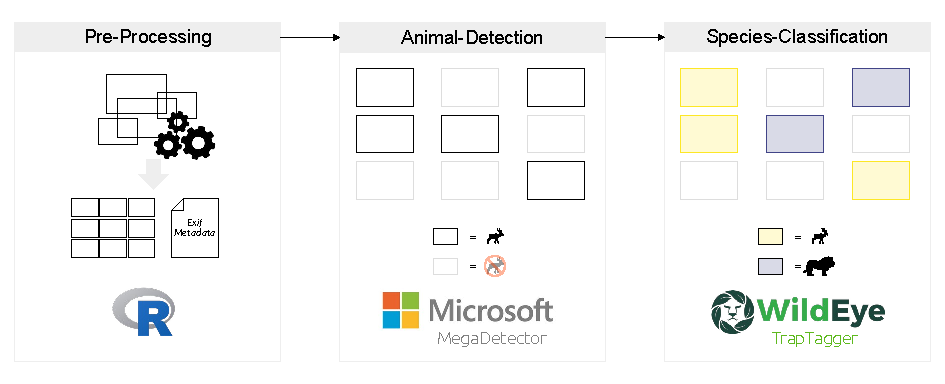
\includegraphics[width = \textwidth]{Figures/CameratrapPipeline}
  \caption{Automated processing pipeline for the cameratrap data. In a first
  step, cameratrap images are preprocessed. This includes the equalization of
  image dimensions, extraction of EXIF-metadata, as well as the assignment of a
  spatial location to each image. In a second step, the pre-processed data is
  fed into Microsoft's MegaDetector, which allows separating empty images from
  images that contain animals. Images with animals are finally processed through
  TrapTagger, which facilitates an AI-aided classification of animals to the
  species level.}
  \label{CameratrapPipeline}
\end{center}
\end{figure}

\section{Supervised Theses}
\label{Supervised}

During the course of my PhD, I had the opportunity to co-supervise two master
students together with my main supervisor, Dr. Gabriele Cozzi. Here, I'd like to
briefly summarize the two students' theses and explain how they embed into my
own work and potentially the work I will conduct during my PostDoc.

\begin{itemize}

  \item \textbf{Factors Influencing Phase-Specific Movement and Activity
  Patterns of African Wild Dogs (by Megan Robinson): } The first thesis was
  conducted by Megan Robinson, who joined our research group in June 2022. Megan
  previously worked as a research assistant for BPC and later embarked as a
  master student in the program for quantitative environmental sciences at the
  University of Zurich. Megan's primary research objective was to quantify
  differences in movement behavior and activity patterns of AWDs during
  residence and dispersal. For this, Megan used GPS and Activity data obtained
  on 33 resident and 19 dispersing AWDs, which she linked to observations
  recorded by staff members in the field to segment the collected data into four
  behavioral movement modes. Specifically, she differentiated between the
  resident phase, when individuals are with the natal pack; the exploratory
  phase, when prospecting individuals may leave the pack for short exploratory
  forays but eventually return to the pack; the transient dispersal phase, when
  dispersing individuals leave their natal pack forever, and the settlement
  phase, during which a newly formed group establishes a new territory. She then
  applied generalized linear mixed-effects models to compare step-lengths,
  turning-angles, and average activity between phases, while holding constant
  for several other factors, including habitat cover, group-size, and
  moon-illumination. Her results revealed that individuals in the exploratory,
  transience, and settlement phase covered significantly larger daily distances
  and exhibited higher average activity than residents (\Cref{MasterTheses}a).
  These differences were particularly pronounced during transience, when
  dispersers cover long distances in a short amount of time. Megan also found
  that AWD activity was positively correlated with moon illumination at night,
  irrespective of the animals' behavioral movement mode. During my PostDoc, I
  envision to build on these insights and further investigate differences
  between resident and dispersing wild dogs via iSSFs. My goal is to further
  assess if observed differences are limited to differences in animals' movement
  behavior (i.e. their movement kernel) or if there are equally relevant
  differences in their habitat-selection function (habitat preferences).

  \item \textbf{Spatial Analysis of Wild Animal Populations in Northern Botswana
  Using Camera Traps Data (by Rapha{\"e}l Destriau):} The second co-supervised
  thesis was conducted by Rapha{\"e}l Destriau, who joined our research group as
  an external student from the Ecole Polytechnique Federale in Lausanne.
  Rapha{\"e}l's background was in engineering, yet he was dedicated to expand
  his expertise in ecology. To accommodate both his expertise and interest, we
  developed a two-stage master thesis, which started with an engineering
  component and later culminated in an ecological analysis. The goal of this
  thesis was to expand on my previously developed processing pipeline to process
  cameratrap data and to conduct a preliminary occupancy analysis on several key
  species. In the first stage, Raph expanded the pipeline and implemented a
  semi-automated workflow to annotate cameratrap images and classify species
  using artificial intelligence. For this, Raph employed an already-existing
  open-source software called \texttt{TrapTagger}
  (\url{www.wildeyeconservation.org}) which provided several pre-trained neural
  networks to detect and classify large mammal species from cameratrap images.
  To benchmark the performances of the available models, Raph manually compiled
  a large validation-dataset that allowed him to compute confusion matrices for
  each available model. Based on these results, Raph developed a
  ``best-practices'' guide that facilitates minimizing potential errors due to
  misclassifications (\Cref{MasterTheses}b), while maximizing the efficiency at
  which data can be processed. In a second stage, Raph utilized the
  automatically processed cameratrap data and applied occupancy models to derive
  species-habitat associations for several species that we believed could
  influence AWDs. The list of modeled species included main AWD prey species
  such as impala (\textit{Aepyceros melampus}), lechwe (\textit{Kobus leche}),
  kudu (\textit{Tragelaphus strepsiceros}), and main AWD competitors such as
  lions (\textit{Panthera leo}), and hyenas (\textit{Crocuta crocuta}). His
  findings suggested significant associations between occupancy and
  environmental factors (e.g. distance to permanent water, vegetation cover,
  proximity to human activity) during the dry season, yet only weak associations
  during the wet season, suggesting either complex ecological dynamics during
  this period or a lack of appropriate spatial information that results in
  stronger species-habitat associations. Raph's thesis laid the foundation for
  an effective pipeline to process additional cameratrap data obtained in
  Botswana, as well as to prepare spatially explicit raster layers that
  represent the distribution of several species that are likely to affect wild
  dog dispersal. During my PostDoc, I plan to rerun Raph's occupancy models
  using updated cameratrap data and to predict spatial layers that can then be
  used as additional covariates in the AWD dispersal model to render the
  influence of competitors and prey on the dispersal behavior of AWDs.

\end{itemize}

\begin{figure}[htpb]
\begin{center}
  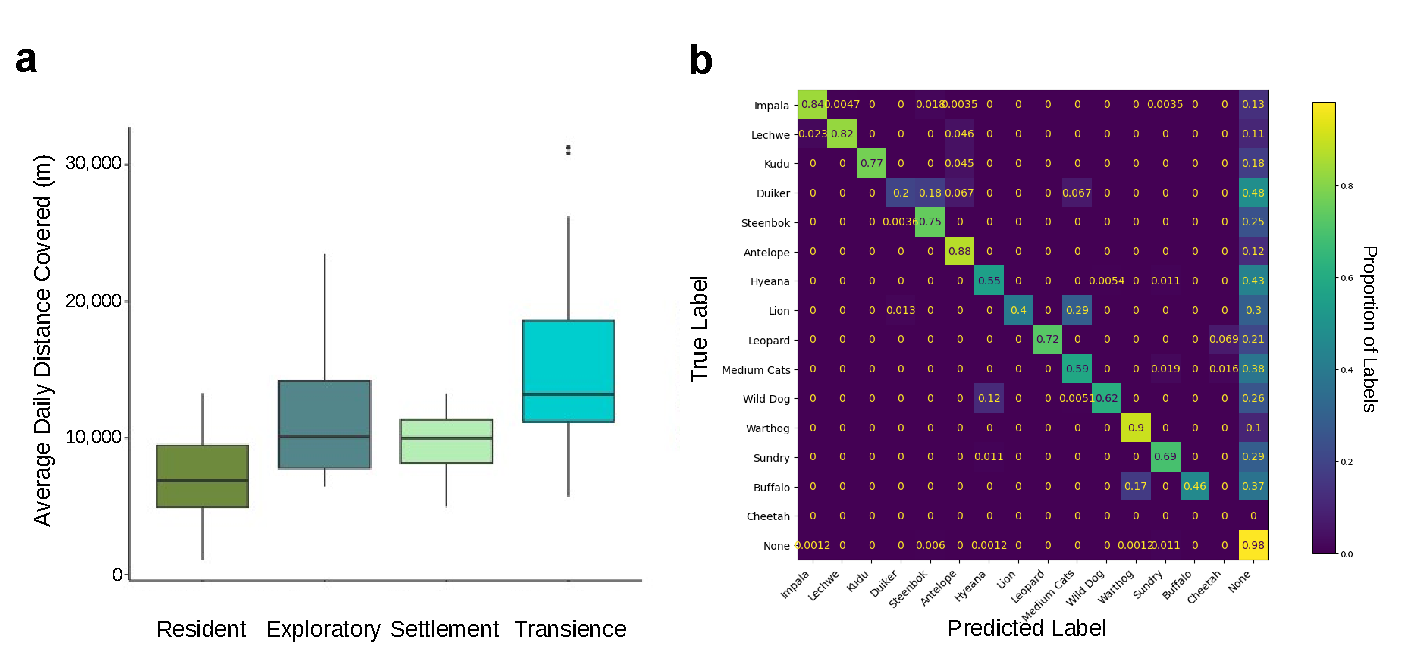
\includegraphics[width = \textwidth]{Figures/MasterTheses}
  \caption{(a) Results from Megan Robinson's master thesis on differences in
  movement behavior of AWDs depending on their behavioral mode / phase. (b)
  Confusion matrix of predicted vs. true labels as obtained from Rapha{\"e}l
  Destriau's thesis, in which he assessed the reliability of TrapTagger to
  correctly assign species labels to cameratrap images.}
  \label{MasterTheses}
\end{center}
\end{figure}

\section{R-Packages}

During the course of my PhD, I developed four small \texttt{R}-packages that
provided useful functionalities for my own work. The packages are available on
GitHub (\url{https://github.com/DavidDHofmann}) and can be installed via the
\texttt{devtools} package. I will here briefly summarize each package's
functionality:

\begin{itemize}

  \item \texttt{video2pic}: \texttt{video2pic} is an \texttt{R}-package that
  allows extracting still frames from a video. In contrast to existing packages,
  the frame-extraction algorithm is implemented in Python, which improves
  efficiency. The ability to extract still images from videos is particularly
  useful in cameratrapping studies, where videos of animals need to be converted
  into still images for classification.

  \item \texttt{floodmapr}: \texttt{floodmapr} is an \texttt{R}-package that
  allows downloading and classifying MODIS MCD43A4 satellite imagery into binary
  maps of dryland and water cover. The classification algorithm is based on
  \citet{Wolski.2017} and currently only applicable for the extent of the
  Okavango Delta. The package handles all data download, as well as the
  necessary processing steps to obtain a ``floodmap'' of the Okavango Delta for
  any desired date.

  \item \texttt{rainmapr}: \texttt{rainmapr} is an \texttt{R}-package that
  allows downloading spatially mapped precipitation estimates from the CHIRPS
  database \citep{Funk.2015}. CHIRPS provides precipitation data dating back to
  1981 at daily or monthly temporal resolutions and spatial resolutions of up to
  0.05\degree.

  \item \texttt{riversim}: \texttt{riversim} is an \texttt{R}-package that
  provides functionalities to simulate river networks. Comparable algorithms to
  simulate land-cover or land-use patterns already exist (e.g., \texttt{NLMR},
  \citealp{Sciaini.2018} or \texttt{gstat}, \citealp{Pebesma.2004}), yet none of
  them achieves realistic looking river systems. The ability to simulate river
  networks is useful for ecological simulation studies, where rivers are assumed
  to play an important role. The original simulation algorithm was developed by
  a reddit user (``TalksInMaths''), yet I translated it into \texttt{R}.

\end{itemize}

\begin{figure}[htpb]
\begin{center}
  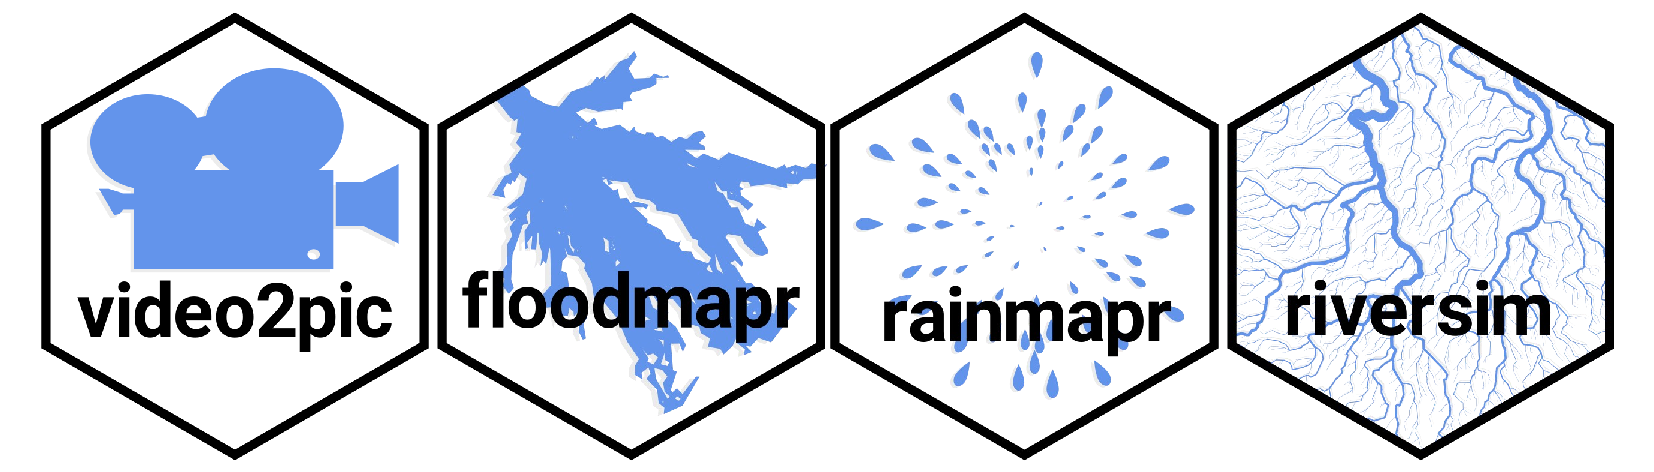
\includegraphics[width = \textwidth]{Figures/Packages}
  \caption{Logos of the \texttt{R}-packages that I developed during the course
  of my PhD.}
  \label{Packages}
\end{center}
\end{figure}

\ifSubfilesClassLoaded{%
  \newpage
  \begin{singlespacing}
  \ifthenelse{\boolean{usebiblatex}}{
    \begin{refcontext}[sorting=nyt]
    \printbibliography
    \end{refcontext}
  } {
    \bibliography{../LiteratureBibtex}%
  }
\end{singlespacing}
}{}

\end{document}
